\section{Methodology}

\subsection{Proposed Technology Stacks}
In this section different technology stacks will be presented, all of which meet the requirements as detailed in the previous section.

\subsubsection{NVIDIA CloudXR (+ NVIDIA Quadro on Azure)}
\begin{figure}[h!]
\caption{Overview of NVIDIA CloudXR Prototype \parencite{cloudxr}}
\label{fig:pr0}
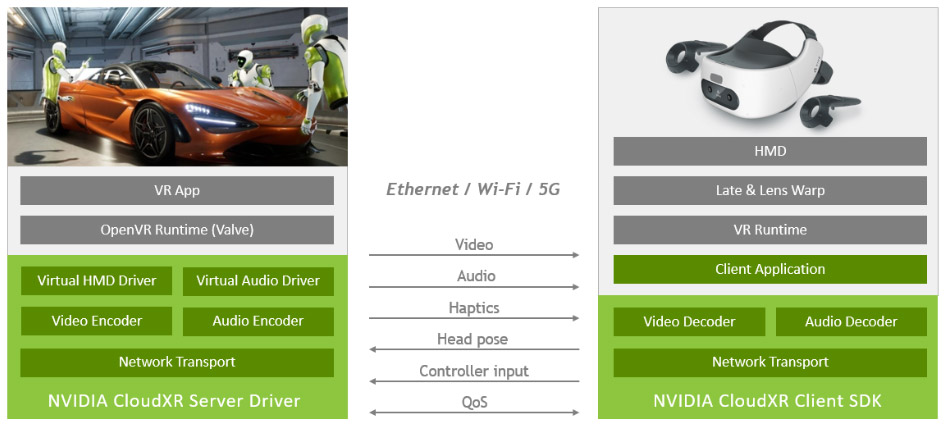
\includegraphics[scale=0.45]{nvidia-cloudxr-diagram}
\end{figure}

The CloudXR SDK from NVIDIA offers a complete solution package to stream VR/AR experiences from server to client. As the only complete package in this list it is a good starting point to create a cloud \acrshort{vr} streaming prototype. Since Azure is the chosen cloud provider of Thales, one of the major stakeholders, the idea would be to deploy this tech stack there. \\
\newline
\begin{varwidth}[t]{.5\textwidth}
\renewcommand\labelitemi{+}
\textbf{Pros:}
\begin{itemize}
\item Only complete solution
\item Increased prototyping speed
\item Custom made for streaming \acrshort{vr} content
\item Works with cutting-edge \acrshort{gpu}'s
\end{itemize}
\end{varwidth}
\hspace{4em}
\begin{varwidth}[t]{.5\textwidth}
\renewcommand\labelitemi{-}
\textbf{Cons:}
\begin{itemize}
\item Forced to use NVIDIA products
\item Not guaranteed to get access to solution (Have to apply to NVIDIA)
\item Limited control about the solution
\item Limited documentation about the solution, since it is brand new
\end{itemize}
\end{varwidth}

\newpage

\subsubsection{WebRTC Prototype 1}
\begin{figure}[h!]
\caption{Overview of WebRTC Prototype 1}
\label{fig:pr11}
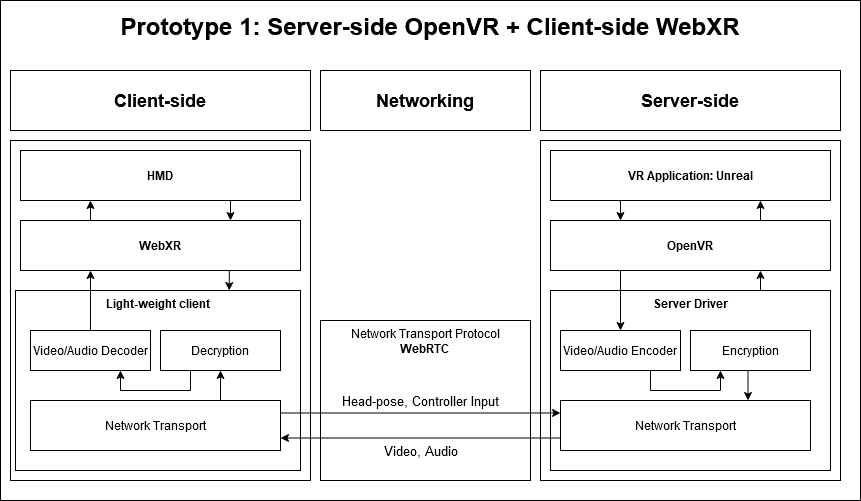
\includegraphics[scale=0.5]{CloudVR_PR1_1}
\end{figure}

WebRTC is one of the premier web technologies to enable real time communications. Since it allows for streaming video and generic data it is a good candidate to create a cloud \acrshort{vr} streaming prototype, because it can transfer both the video and input data. As it has a focus on real time communication it is optimized to reduce latency by default, however it is unclear if this is enough optimization by itself to support streaming \acrshort{vr} content. To enable the application to run "normally" OpenVR will be used to provide a virtual interface of the physical hardware on the removed remote server. By receiving pose updates from the Client and using those updates to create a virtual \acrshort{hmd} the application can be developed like a local VR application. \\
\newline
\begin{varwidth}[t]{.5\textwidth}
\renewcommand\labelitemi{+}
\textbf{Pros:}
\begin{itemize}
\item Works for the majority of \acrshort{hmd}'s + platforms
\item Mostly Open source
\item WebRTC is well documented and supported
\end{itemize}
\end{varwidth}
\hspace{4em}
\begin{varwidth}[t]{.5\textwidth}
\renewcommand\labelitemi{-}
\textbf{Cons:}
\begin{itemize}
\item Lower performance Web Technologies (but there are native clients for all major platforms available)
\item Higher complexity due to more components
\item OpenVR + WebXR are sparsely documented
\end{itemize}
\end{varwidth}

\subsubsection{WebRTC Prototype 2}
\begin{figure}[h!]
\caption{Overview of WebRTC Prototype 2}
\label{fig:pr12}
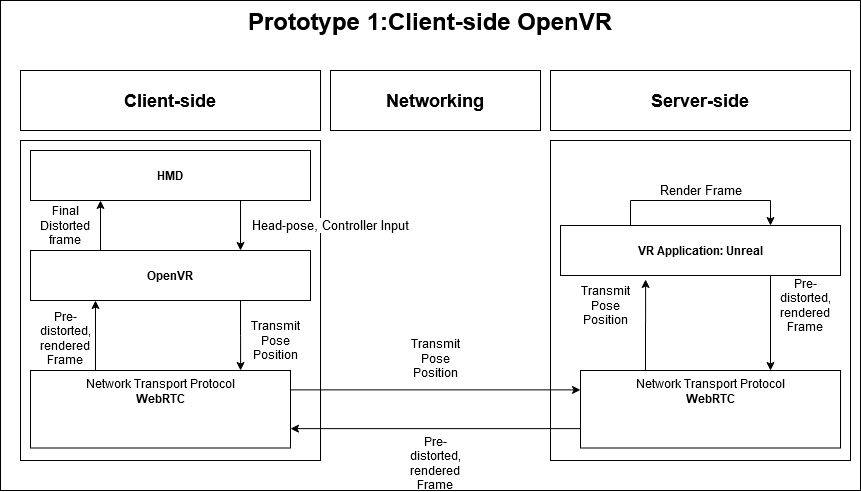
\includegraphics[scale=0.5]{CloudVR_PR1_2}
\end{figure}

This protoype candidate is similar in design to the previous one, in the sense that it uses WebRTC for networking and OpenVR for interacting with a \acrshort{hmd}. The key difference is that the application on the server does not know it is rendering specifically for VR. All the distortion operations, to generate an image for the \acrshort{hmd} from the recieved frame, will be done on the client-side with OpenVR. \\
\newline
\begin{varwidth}[t]{.5\textwidth}
\renewcommand\labelitemi{+}
\textbf{Pros:}
\begin{itemize}
\item Less complex than previous solution due to less components 
\item Utilizes OpenVR to gain access to HMD's: The type/manufacturer does not matter
\end{itemize}
\end{varwidth}
\hspace{4em}
\begin{varwidth}[t]{.5\textwidth}
\renewcommand\labelitemi{-}
\textbf{Cons:}
\begin{itemize}
\item Will only work in a very specific set up
\end{itemize}
\end{varwidth}